\documentclass[final, landscape]{beamer}

\usepackage[size=a0, orientation=landscape, scale=1.4]{beamerposter}
\usepackage{graphicx}
\usepackage{booktabs}
\usepackage{amsmath,amssymb}
\usepackage{multicol}
\usepackage{tikz}
\usetikzlibrary{shapes.geometric, arrows.meta, positioning, fit}

% --- Theme ---
\usetheme{default}
\setbeamertemplate{navigation symbols}{}
\setbeamertemplate{caption}[numbered]

% --- Colors ---
\definecolor{PrimaryBlue}{RGB}{0, 74, 153}
\definecolor{LightGray}{RGB}{240, 240, 240}

\setbeamercolor{headline}{fg=white, bg=PrimaryBlue}
\setbeamercolor{block title}{fg=white, bg=PrimaryBlue}
\setbeamercolor{block body}{fg=black, bg=LightGray}
\setbeamercolor{footline}{fg=white, bg=PrimaryBlue}

% --- Block style ---
\setbeamertemplate{block begin}{
  \vskip0.5ex
  \begin{beamercolorbox}[rounded=true, shadow=true, leftskip=1em, colsep*=0.3ex]{block title}
    \usebeamerfont{block title}\insertblocktitle
  \end{beamercolorbox}
  \vskip0.3ex
  \begin{beamercolorbox}[rounded=true, shadow=true, leftskip=1em, rightskip=1em, colsep*=0.3ex]{block body}
    \vskip0.3ex
}
\setbeamertemplate{block end}{
  \end{beamercolorbox}
  \vskip0.5ex
}

% --- Headline ---
\setbeamertemplate{headline}{
  \begin{beamercolorbox}[wd=\paperwidth]{headline}
    \vskip1.2cm
    \centering
    {\Huge\bfseries Extracting Recipes from Cooking Videos\\[0.3cm]
     using V-JEPA2 Embeddings}\\[0.7cm]
    {\Large Michelangelo Bettini \\ \Large Pablo Landrove Pérez-Gorgoroso}\\[0.3cm]
    {\large Università della Svizzera Italiana}\\[0.3cm]
    {\normalsize \texttt{Group P}}
    \vskip1.2cm
  \end{beamercolorbox}
}

% --- Footline ---
\setbeamertemplate{footline}{
  \begin{beamercolorbox}[wd=\paperwidth]{footline}
    \vskip0.5cm
    \centering
    {\normalsize Computer Vision Course Project, 2026}
    \vskip0.5cm
  \end{beamercolorbox}
}

% ============================================================
\begin{document}
\begin{frame}[t]

% pipeline block defined inline — opened inside middle column below
% (placeholder comment, actual block is in middle column)
\begin{columns}[t]

% ---- LEFT COLUMN ----
\begin{column}{0.22\paperwidth}

  \begin{block}{Introduction}

    \textbf{V-JEPA 2} provides an accessible way to encode complex physical
    interactions in videos without fine-tuning the visual backbone.

    Understanding \textbf{egocentric cooking videos} is challenging:
    first-person footage captures natural kitchen activities but suffers
    from clutter, and difficult recognition of objects.

    \vskip0.3em
    We propose a \textbf{two-stage pipeline}:
    \begin{enumerate}
      \item \textbf{Relevance filtering} — separate cooking actions
            from background events.
      \item \textbf{Action classification} — fine-grained verb/noun
            recognition on relevant clips.
    \end{enumerate}

    \vskip0.3em
    We exploit \textbf{V-JEPA2 embeddings} and train a lightweight temporal
    classifier on top, keeping compute requirements minimal.
  \end{block}

  \begin{block}{Dataset: EPIC-KITCHENS-100}
    \begin{itemize}
      \item \textbf{407 embedded videos}, split into \textbf{170,007}
            temporal blocks
      \item \textbf{1024-D V-JEPA2 embeddings} per 64-frame block
      \item \textbf{116,812} blocks overlap an annotation; \textbf{53,195}
            are background/unannotated
      \item \textbf{5,988} relevant verb--noun action-pair classes used by
            the action head
    \end{itemize}

    \vskip0.3em
    \begin{center}
    \begin{tabular}{lr}
      \toprule
      Block label & Fraction \\
      \midrule
      Relevant    & 60.0\% \\
      Irrelevant/background  & 40.0\% \\
      \bottomrule
    \end{tabular}
    \end{center}

  \end{block}

  \begin{block}{Why V-JEPA2-small?}
    We use the \textbf{small} variant of V-JEPA2 (ViT-L backbone,
    $\approx$307M parameters). Its compact footprint makes local inference
    feasible on a \textbf{MacBook Pro} or consumer laptop with sufficient GPU
    RAM. For this project we used \textbf{cloud compute} to embed the dataset
    in reasonable time, then trained the classifier on Apple MPS.
  \end{block}

\end{column}

% ---- MIDDLE COLUMN (wide — pipeline + details) ----
\begin{column}{0.52\paperwidth}

  \begin{block}{Pipeline Overview}
    \centering
    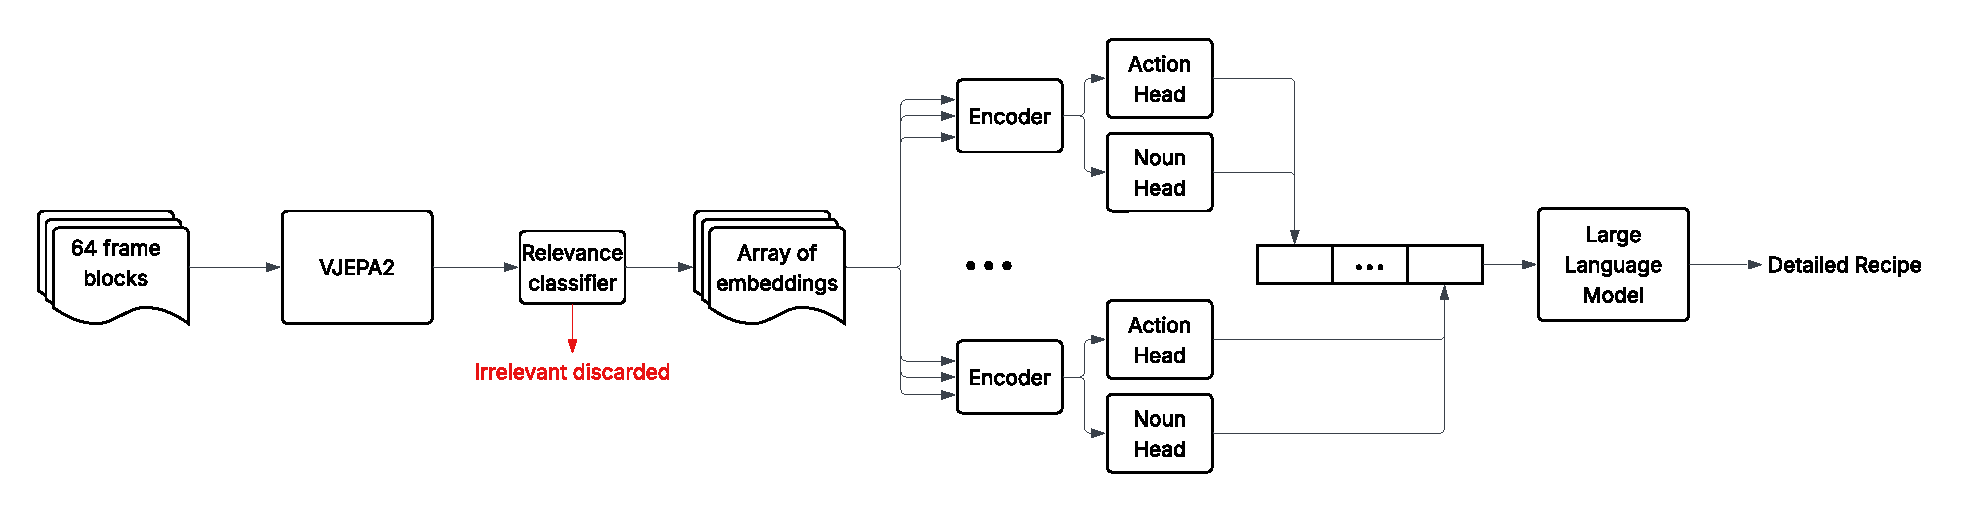
\includegraphics[width=\linewidth]{figures/pipeline2}
  \end{block}

  \begin{block}{Classification Heads}
    A shared temporal encoder reads a 7-block window (radius 3). Each
    1024-D embedding is projected to 768 dimensions, learned positional
    encodings are added, and a 2-layer, 8-head TransformerEncoder aggregates
    context. Missing neighbors at video boundaries are zero-padded and masked.

    \vskip0.3em
    The center token feeds four MLP heads: \textbf{relevance} (binary),
    \textbf{verb}, \textbf{noun}, and \textbf{action pair}. Relevance is
    trained on all blocks; action losses are masked to valid relevant blocks.

    \vskip0.3em
    At inference, action prediction combines action, verb, and noun log
    probabilities with a smoothed verb--noun pair prior ($w=0.25$). A
    3-seed ensemble (42, 123, 999) averages logits before decoding.
  \end{block}

  \vskip0.5em
  \begin{center}
    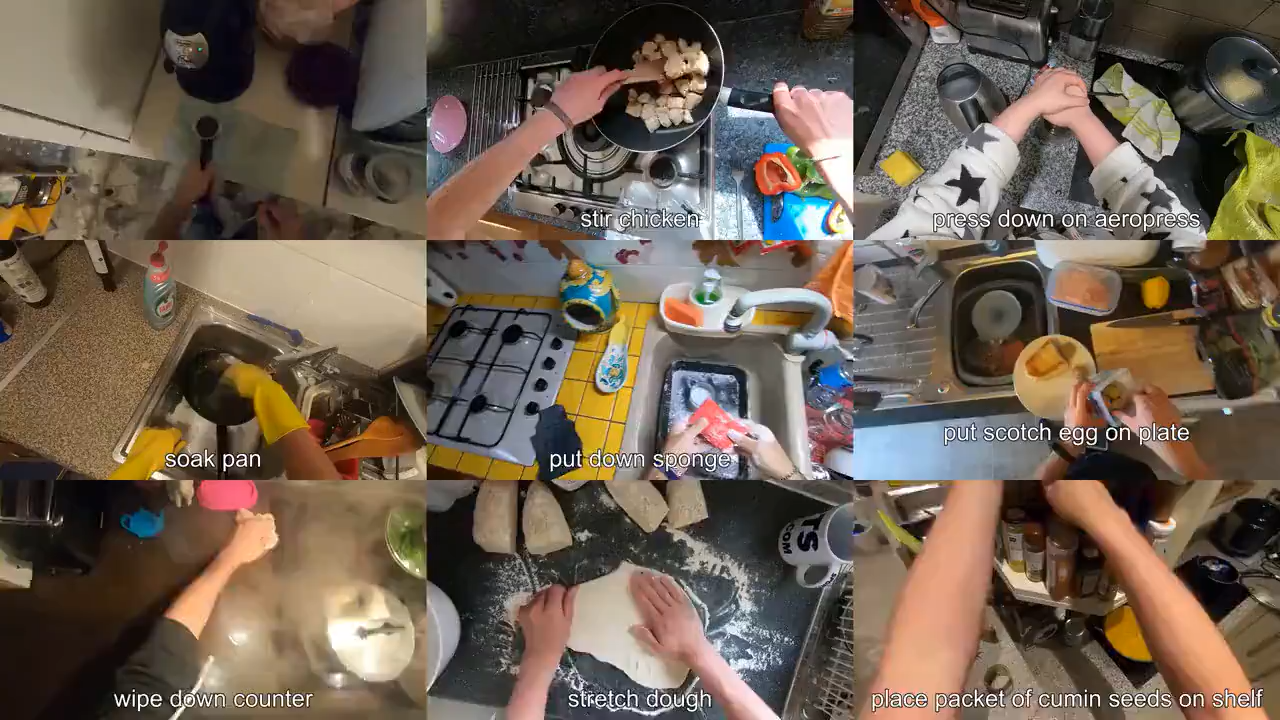
\includegraphics[width=\linewidth]{figures/kitchen}
  \end{center}

\end{column}

% ---- RIGHT COLUMN ----
\begin{column}{0.22\paperwidth}

  \begin{block}{Why a Transformer Encoder?}
    A single block provides only a narrow temporal context.
    A Transformer encoder attends across the full sequence of block
    embeddings, aggregating multi-window evidence before the center-token
    heads decide relevance and action labels.
  \end{block}

  \begin{block}{Results}
    \begin{center}
    \begin{tabular}{lcc}
      \toprule
      Metric & Val & Test \\
      \midrule
      Relevance accuracy & 82.9\% & 84.0\% \\
      Relevance F1       & 86.1\% & 87.0\% \\
      Verb accuracy      & 74.4\% & 77.3\% \\
      Noun accuracy      & 77.7\% & 80.3\% \\
      Exact action       & 73.0\% & 75.8\% \\
      \bottomrule
    \end{tabular}
    \end{center}

    \vskip0.3em
    Action scores are measured after the relevance gate on true relevant
    blocks. With oracle relevance, test exact-action accuracy reaches
    \textbf{84.4\%}; on predicted relevant blocks it is \textbf{87.2\%}.
  \end{block}

  \begin{block}{LLM Post-Processing}
    The action classifier outputs a \textbf{sequence of (verb, noun) pairs}
    aligned to video blocks.
    We pass this sequence to \textbf{Llama 3.2} which
    synthesizes the raw event list into a fluent, human-readable recipe:
    coherent steps, resolved repetitions, and natural prose.

    \vskip0.3em
    This bridges the gap between frame-level predictions and
    interpretable cooking instructions.
  \end{block}

  \begin{block}{Conclusion}
    \begin{itemize}
      \item \textbf{Two-stage design} (relevance + classification) cuts
            background noise before fine-grained prediction.
      \item \textbf{Transformer encoder} provides multi-block temporal
            context with minimal added parameters.
      \item \textbf{LLM post-processing} turns sparse event sequences
            into readable recipes.
      \item Pipeline runs on consumer hardware with no backbone tuning.
    \end{itemize}
  \end{block}

\end{column}

\end{columns}
\end{frame}
\end{document}
